\documentclass[11pt]{article}
\usepackage[margin=1in]{geometry}
\usepackage{hyperref}
\usepackage{array}
\usepackage{tabularx}
\usepackage{enumitem}
\usepackage{xcolor}
\usepackage{listings}
\usepackage{pgfplots}
\pgfplotsset{compat=1.18}
\renewcommand{\arraystretch}{1.28}
\setlength{\tabcolsep}{6pt}
\newcolumntype{Y}{>{\raggedright\arraybackslash}X}

\lstset{
  basicstyle=\ttfamily\small,
  breaklines=true,
  frame=single,
  columns=fullflexible
}

\title{HR Resume RAG Assistant: Implementation Report}
\author{}
\date{}

\begin{document}
\maketitle

\section{Project Summary}

This project implements a chat-first HR assistant for resume screening over the Kaggle Resume Dataset. The system focuses on the \texttt{BANKING} and \texttt{INFORMATION-TECHNOLOGY} domains and indexes only those two resume groups.

The key design choice is to use structured candidate profiles plus section-level evidence retrieval instead of generic semantic chunking. Resumes are already semi-structured, so the system extracts one profile per candidate and keeps natural sections such as Summary, Skills, Experience, Education, and Certifications as evidence.

For source code, setup instructions, and implementation details, see: \url{https://github.com/nutbred/cv-chatbot}.

\section{HR Workflow Research and Product Assumptions}

This section documents the product research and assumptions behind the implementation. The target user is an HR or recruiting user with limited technical background. The system therefore prioritizes a chat-first workflow, short explanations, visible evidence, and clear warnings over a purely technical search interface.

\subsection{User Context}

Typical HR questions are natural-language screening tasks:

\begin{itemize}[leftmargin=*]
  \item Find IT candidates with backend, SQL, and at least one year of experience.
  \item Find Banking candidates with KYC and AML experience.
  \item Explain why a candidate is weak for a Power BI-heavy role.
  \item Show stretch candidates if they are close enough.
  \item Compare candidates and explain tradeoffs.
\end{itemize}

The product should therefore behave like an assistant that helps HR reason about fit, not only a vector search demo.

\subsection{Core Assumptions}

\begin{center}
\begin{tabularx}{\linewidth}{|p{0.34\linewidth}|Y|}
\hline
\textbf{Assumption} & \textbf{Product decision} \\
\hline
HR needs explanations, not only IDs & Return matched skills, gaps, recommendation, and CV evidence \\
\hline
CVs are already structured & Use candidate profiles plus section evidence, not generic semantic chunks \\
\hline
Hiring criteria can be flexible & Support flexible and strict screening modes \\
\hline
Banking and IT use many acronyms & Add glossary normalization and BM25 retrieval \\
\hline
LLMs can hallucinate & Keep retrieval/ranking deterministic and only let the LLM rewrite grounded evidence \\
\hline
Company names are anonymized & Do not use company prestige as a ranking signal \\
\hline
\end{tabularx}
\end{center}

\subsection{Design Tradeoffs}

\begin{center}
\begin{tabularx}{\linewidth}{|p{0.31\linewidth}|Y|}
\hline
\textbf{Decision} & \textbf{Reasoning} \\
\hline
Structured profiles first & HR evaluates candidate-level suitability rather than isolated paragraphs \\
\hline
Section evidence second & Skills and experience evidence should be traceable to natural CV sections \\
\hline
Hybrid FAISS + BM25 & Embeddings handle broad language; BM25 protects exact terms like KYC, AML, SQL, BE, FE \\
\hline
Heuristic MVP + optional LLM & The app runs without API cost, but can use DeepSeek when available \\
\hline
Optional LlamaParse & pypdf works for the current PDFs; LlamaParse is useful for scanned or complex future PDFs \\
\hline
Flexible default & Recruiters often want promising near matches \\
\hline
Strict toggle & Some requirements are hard filters and must exclude uncertain candidates \\
\hline
\end{tabularx}
\end{center}

\subsection{HR Reasoning Model}

The assistant uses three buckets:

\begin{itemize}[leftmargin=*]
  \item Strong Match: domain, required skills, and measurable requirements are supported by evidence.
  \item Near Match: a measurable requirement is missing, but compensating evidence exists.
  \item Not Recommended: core requirements are missing and there is not enough compensation.
\end{itemize}

For example, a candidate with three years of experience should not be labeled a strong match for a five-year requirement. However, if the candidate has highly aligned projects and the requested tools, flexible mode can show the candidate as a near match with a clear caveat.

\subsection{Why Prestige and Scope Signals Matter}

Prestige or high-scope experience can be useful when a candidate misses a measurable requirement but may still deserve review. For example, a candidate with three years of experience instead of five may still be a reasonable near match if the CV shows unusually strong compensating evidence:

\begin{itemize}[leftmargin=*]
  \item experience at a recognized bank, fintech, or technology company;
  \item senior or high-responsibility title for the experience level;
  \item ownership of regulated, production, or large-scale systems;
  \item domain-aligned projects that directly match the role;
  \item certifications or repeated evidence across multiple experience bullets.
\end{itemize}

This signal should not turn a missing hard requirement into a strong match by itself. It is best used to explain why a candidate is a near match rather than ignored completely.

For the current Kaggle resumes, many employer names are anonymized as \texttt{Company Name}, so the implementation does not use company prestige as a primary scoring feature. Instead, it uses more reliable compensation signals available in the text: seniority, project ownership, certifications, tool overlap, and domain alignment. For uploaded real-world CVs with visible employer names, prestige or company-scope could be added as an optional, transparent signal.

\subsection{Edge-Case Policies}

\begin{center}
\begin{tabularx}{\linewidth}{|p{0.34\linewidth}|Y|}
\hline
\textbf{Edge case} & \textbf{Policy} \\
\hline
Three years vs five years requested & Flexible mode can show near match; strict mode excludes \\
\hline
Skill appears only in education & Lower confidence and suggest verification \\
\hline
Right skills but wrong domain & Domain filter blocks if domain is explicit \\
\hline
Right domain but missing core tool & Near match or not recommended depending on compensation \\
\hline
Missing or unclear dates & Show uncertainty; strict mode excludes if years are required \\
\hline
BE abbreviation & Warn that it can mean Backend Engineering or Bachelor of Engineering \\
\hline
B.E. in education context & Treat as degree, not backend \\
\hline
Lowercase ``be'' & Ignore as abbreviation \\
\hline
PowerBI / Power BI / BI & Normalize as related evidence \\
\hline
Scanned PDF & Mark low text and optionally use LlamaParse \\
\hline
LLM unavailable & Fall back to deterministic grounded answer \\
\hline
\end{tabularx}
\end{center}

\subsection{Risks and Mitigations}

\begin{center}
\begin{tabularx}{\linewidth}{|p{0.31\linewidth}|Y|}
\hline
\textbf{Risk} & \textbf{Mitigation} \\
\hline
LLM hallucination & LLM receives only retrieved evidence and is instructed not to invent facts \\
\hline
Keyword stuffing & Evidence snippets show whether skills appear in real work context \\
\hline
Acronym ambiguity & Glossary and clarification notes \\
\hline
Incorrect years estimate & Years are labeled as estimates and uncertain fields are exposed \\
\hline
Over-filtering good candidates & Flexible mode surfaces near matches \\
\hline
Under-filtering hard requirements & Strict mode excludes missing or uncertain hard criteria \\
\hline
\end{tabularx}
\end{center}

\section{Technology Stack}

\begin{center}
\begin{tabularx}{\linewidth}{|p{0.31\linewidth}|Y|}
\hline
\textbf{Layer} & \textbf{Tooling} \\
\hline
UI & Streamlit \\
\hline
CLI & Python argparse \\
\hline
PDF parsing & pypdf \\
\hline
Optional enhanced parsing & LlamaParse \\
\hline
LLM integration & OpenAI SDK-compatible DeepSeek API \\
\hline
Embedding retrieval & sentence-transformers/all-MiniLM-L6-v2 \\
\hline
Vector index & FAISS \\
\hline
Lexical retrieval & BM25 with rank-bm25 \\
\hline
Artifacts & JSONL, FAISS index, BM25 pickle \\
\hline
\end{tabularx}
\end{center}

\section{Workflow}

\begin{enumerate}[leftmargin=*]
  \item Discover PDFs from only \texttt{data/BANKING} and \texttt{data/INFORMATION-TECHNOLOGY}.
  \item Parse PDFs locally with \texttt{pypdf}.
  \item Optionally use LlamaParse for low-text or complex uploaded PDFs.
  \item Extract one candidate profile per resume.
  \item Extract section/page evidence blocks for citations.
  \item Build FAISS embeddings and a BM25 lexical index.
  \item Interpret HR queries into domain, role, skills, years, strict/flexible mode, and candidate IDs.
  \item Rank candidates into Strong Match, Near Match, or Not Recommended.
  \item Return deterministic output or optional LLM-written HR response grounded in retrieved evidence.
\end{enumerate}

\section{Dataset and Artifacts}

\begin{center}
\begin{tabularx}{0.82\linewidth}{|Y|r|}
\hline
\textbf{Check} & \textbf{Result} \\
\hline
Total indexed PDFs & 235 \\
\hline
Banking PDFs & 115 \\
\hline
Information Technology PDFs & 120 \\
\hline
Evidence blocks & 1490 \\
\hline
Low-text PDFs detected & 0 \\
\hline
Candidate profiles & 235 \\
\hline
\end{tabularx}
\end{center}

\subsection{Dataset Distribution Plot}

\begin{center}
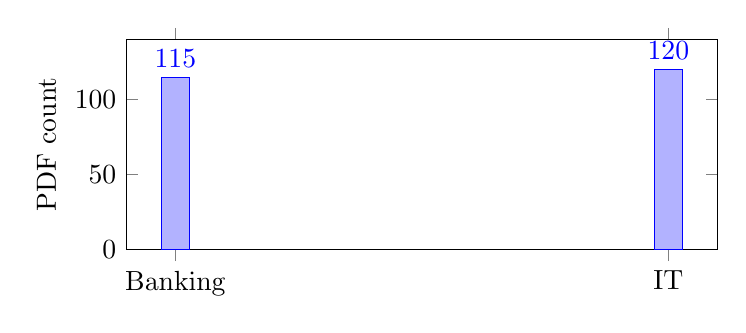
\begin{tikzpicture}
\begin{axis}[
    ybar,
    ymin=0,
    ymax=140,
    ylabel={PDF count},
    symbolic x coords={Banking,IT},
    xtick=data,
    nodes near coords,
    width=0.75\linewidth,
    height=0.35\linewidth
]
\addplot coordinates {(Banking,115) (IT,120)};
\end{axis}
\end{tikzpicture}
\end{center}

\subsection{Artifact Volume Plot}

\begin{center}
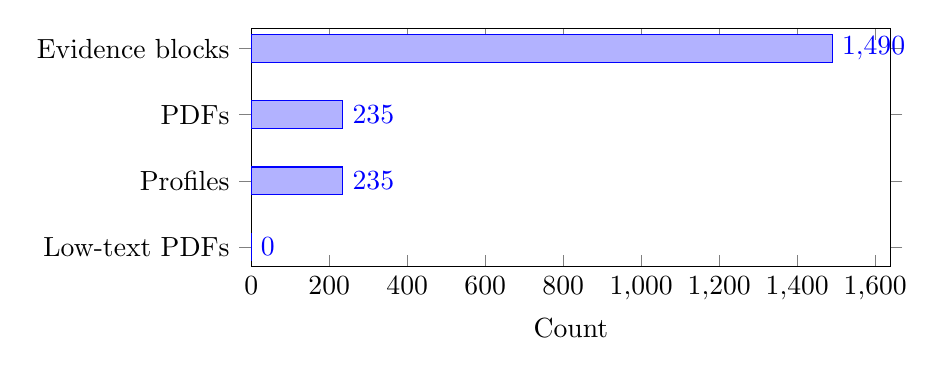
\begin{tikzpicture}
\begin{axis}[
    xbar,
    xmin=0,
    xlabel={Count},
    symbolic y coords={Low-text PDFs,Profiles,PDFs,Evidence blocks},
    ytick=data,
    nodes near coords,
    width=0.8\linewidth,
    height=0.38\linewidth
]
\addplot coordinates {(0,Low-text PDFs) (235,Profiles) (235,PDFs) (1490,Evidence blocks)};
\end{axis}
\end{tikzpicture}
\end{center}

\section{Retrieval Design}

The project uses hybrid retrieval:

\begin{itemize}[leftmargin=*]
  \item Structured filters for domain, strict mode, years, and candidate IDs.
  \item FAISS vector retrieval for broad semantic similarity.
  \item BM25 lexical retrieval for exact acronyms and skills such as KYC, AML, SQL, BE, FE, and Power BI.
\end{itemize}

This hybrid approach is better than pure vector search for resumes because HR queries often contain exact skills, acronyms, tools, and compliance terms.

\section{LLM Usage}

The LLM is optional and explicit. It is used in two places:

\begin{itemize}[leftmargin=*]
  \item \texttt{--use-llm-profile}: extract richer candidate profiles during build.
  \item \texttt{--use-llm}: rewrite grounded retrieval results into an HR-friendly answer.
\end{itemize}

The LLM is not allowed to invent facts. The prompt instructs it to use only the provided structured matches and evidence.

The DeepSeek smoke test returned:

\begin{lstlisting}
LLM_AVAILABLE True
MODEL deepseek-v4-flash
BASE_URL https://api.deepseek.com
RESULT FLASH_OK
\end{lstlisting}

\subsection{LLM Validation Suite}

Additional tests were run with \texttt{deepseek-v4-flash}.

\begin{center}
\begin{tabularx}{\linewidth}{|p{0.25\linewidth}|p{0.35\linewidth}|Y|}
\hline
\textbf{Test} & \textbf{Prompt / action} & \textbf{Result} \\
\hline
Direct smoke & Reply exactly: FLASH\_OK & Returned FLASH\_OK \\
\hline
Banking grounded answer & Find banking candidates with KYC and AML experience & Returned two Banking strong matches with KYC/AML evidence \\
\hline
IT abbreviation answer & Find BE candidates with Java and SQL & Preserved the BE ambiguity warning and returned IT backend matches \\
\hline
Banking near-match answer & Find banking candidates with KYC and AML and at least 20 years experience & Returned near matches with explicit missing KYC or experience gap \\
\hline
LLM profile extraction & One IT resume profile extraction & Returned \texttt{llm+heuristic}; role Information Technology Technician I; 64 skills; 40 tools; 19.0 estimated years; 1 uncertainty note \\
\hline
\end{tabularx}
\end{center}

The LLM is deliberately not the retrieval engine. It only receives retrieved candidates, match buckets, missing requirements, and evidence snippets. This keeps the answer grounded while making the final response easier for HR to read.

\section{Example Prompts and Outputs}

\subsection{Without LLM}

\begin{lstlisting}
python -m hr_resume_rag.cli ask "Find banking candidates with KYC and AML experience" --top-k 2
\end{lstlisting}

Output excerpt:

\begin{lstlisting}
Screening mode: flexible. Found 2 candidate(s).

1. Candidate 11065180 - Strong match (BANKING, 12.5 years)
Matched: Domain: BANKING, AML, KYC
Recommendation: Compliance is a strong match because the CV supports the main requested criteria.

2. Candidate 28989677 - Strong match (BANKING, 5 years)
Matched: Domain: BANKING, AML, KYC
\end{lstlisting}

\subsection{With LLM}

\begin{lstlisting}
python -m hr_resume_rag.cli ask "Find banking candidates with KYC and AML experience" --top-k 2 --use-llm
\end{lstlisting}

Output excerpt:

\begin{lstlisting}
Recruiter Summary - Banking KYC/AML Candidates

Rank 1: Resume ID 11065180 - Strong Match
Why this candidate fits:
- Deep banking domain experience in compliance/operations.
- Explicitly lists KYC and AML in the skills section and demonstrates them in practice.

Rank 2: Resume ID 28989677 - Strong Match
Why this candidate fits:
- Direct AML/KYC compliance role with hands-on compliance experience.
\end{lstlisting}

\subsection{Abbreviation Query}

\begin{lstlisting}
python -m hr_resume_rag.cli ask "Find BE candidates with Java and SQL" --top-k 3
\end{lstlisting}

Output excerpt:

\begin{lstlisting}
Clarification note: BE is ambiguous: Backend Engineering, Bachelor of Engineering.

1. Candidate 83816738 - Strong match (INFORMATION-TECHNOLOGY, 4.2 years)
Matched: Domain: INFORMATION-TECHNOLOGY, Java, SQL, Backend Engineering
\end{lstlisting}

\section{Edge Cases}

\begin{center}
\begin{tabularx}{\linewidth}{|p{0.34\linewidth}|Y|}
\hline
\textbf{Edge case} & \textbf{Handling} \\
\hline
Below required years & Near match in flexible mode, excluded in strict mode \\
\hline
Unclear years & Near match in flexible mode, excluded if strict and years are required \\
\hline
BE abbreviation & Context-aware warning; maps to backend in IT context \\
\hline
B.E. degree & Treated as education context \\
\hline
Lowercase ``be'' & Ignored as abbreviation \\
\hline
KYC/AML exact acronyms & BM25 improves exact matching \\
\hline
PowerBI vs Power BI & Normalized as Power BI / BI evidence \\
\hline
Wrong domain & Domain filter prevents cross-domain results \\
\hline
Missing core skill & Near match or not recommended depending on compensation \\
\hline
Scanned PDF & Low-text detection; optional LlamaParse fallback \\
\hline
LLM key missing or invalid & Fall back to deterministic grounded answer \\
\hline
\end{tabularx}
\end{center}

\section{Evaluation}

Latest evaluation:

\begin{center}
\begin{tabularx}{0.82\linewidth}{|Y|r|}
\hline
\textbf{Metric} & \textbf{Result} \\
\hline
Query count & 15 \\
\hline
Domain precision at 5 & 1.0 \\
\hline
Citation coverage & 1.0 \\
\hline
JSON validity rate & 1.0 \\
\hline
Average latency & 14.144 seconds \\
\hline
Profile count & 235 \\
\hline
\end{tabularx}
\end{center}

\subsection{Evaluation Metrics Plot}

\begin{center}
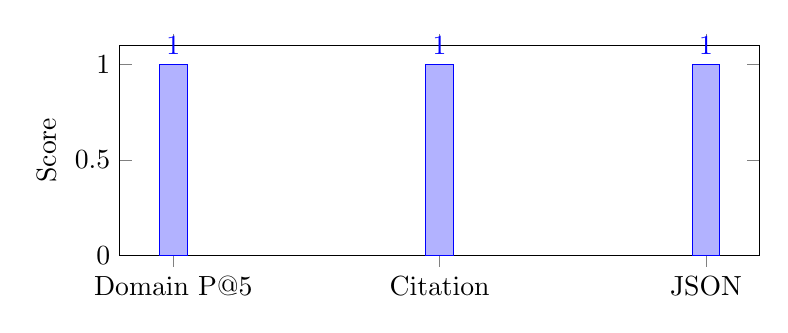
\begin{tikzpicture}
\begin{axis}[
    ybar,
    ymin=0,
    ymax=1.1,
    ylabel={Score},
    symbolic x coords={Domain P@5,Citation,JSON},
    xtick=data,
    nodes near coords,
    width=0.8\linewidth,
    height=0.35\linewidth
]
\addplot coordinates {(Domain P@5,1.0) (Citation,1.0) (JSON,1.0)};
\end{axis}
\end{tikzpicture}
\end{center}

\subsection{Field Coverage Plot}

\begin{center}
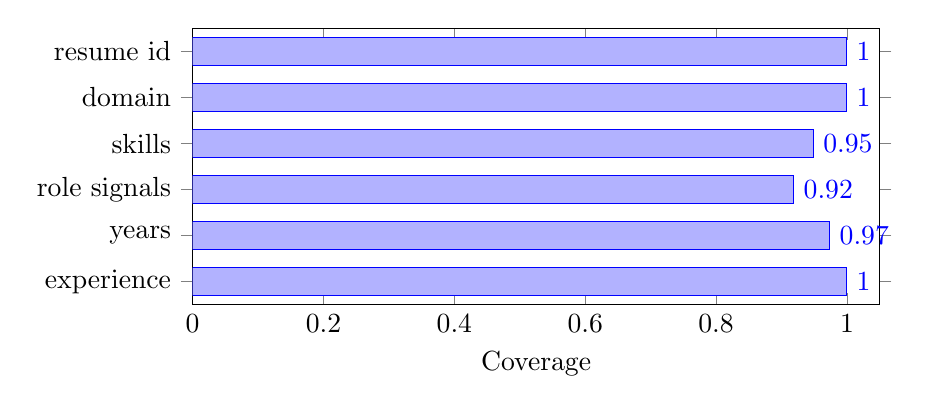
\begin{tikzpicture}
\begin{axis}[
    xbar,
    xmin=0,
    xmax=1.05,
    xlabel={Coverage},
    symbolic y coords={experience,years,role signals,skills,domain,resume id},
    ytick=data,
    nodes near coords,
    width=0.85\linewidth,
    height=0.42\linewidth
]
\addplot coordinates {
  (1.0,experience)
  (0.974,years)
  (0.919,role signals)
  (0.949,skills)
  (1.0,domain)
  (1.0,resume id)
};
\end{axis}
\end{tikzpicture}
\end{center}

\end{document}
